\chapter{RESULT \& ANALYZE OF TEST}\label{cha:result}
TODO!

% ========== GYROTION TEST ==========
\section{Result Accelerometer \& Gyroscope-test}
As described in ~\chapterref{cha:measurements}, two test have been preformed on the accelerometer and gyroscope data with the result presented here.
\subsection{Test I}
The data were gathered as described in~\sectionref{sec:measurement:gyrotion} from the web-page in \figureref{fig:gyrotion} by sending the link of the page. When looking at devices with similar or same hardware you can see differences in measurements, for example here are the accelerometer recordings from 5 iPhone 6 and 1 iPhone 5S:
\begin{figure}[h!]
\centering
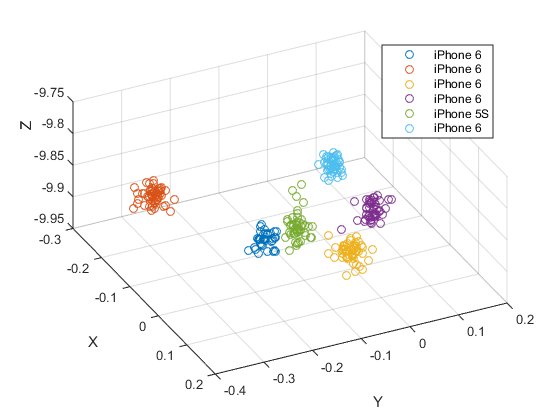
\includegraphics[scale=.7]{img/scatteriPhone}
\caption{Scatter graph on accelerometer recordings of 6 Apple devices}
\label{fig:digraph}
\end{figure}
The conclusion made from this made me ... SKRIV LITE OM RMS, SD, MEAN O LÄGG TILL PASSANDE GRAFER... \\

\subsection{Test II}
The page from Test I was developed by the test-result. The changes that were made is described in~\sectionref{sec:measurement:sensorrec} to improve that analyze data. The changes where improvements that as seen in~\figureref{fig:scatter1m} of six Android devices, that includes measurements for two of the devices with one month apart and you still see the measurements at the same spots.
\begin{figure}[H]
	\centering
	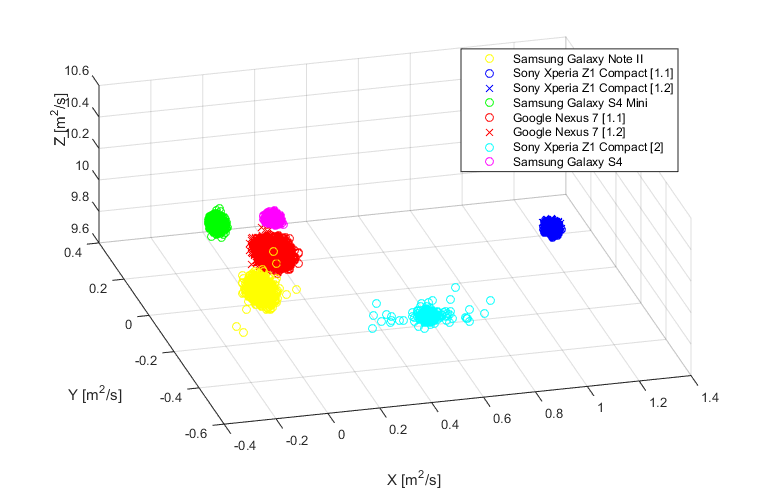
\includegraphics[scale=.7]{img/oneMonth-scatter}
	\caption{Scatter graph on accelerometer recordings of 6 Android devices, where two has one month apart}
	\label{fig:scatter1m}
\end{figure}
Another thing you can see from just these three measurements are that RMS (Root-mean-square) is still no good feature for fingerprinting eaven if the measurements are interpolated over time.
\begin{figure}[H]
	\centering
	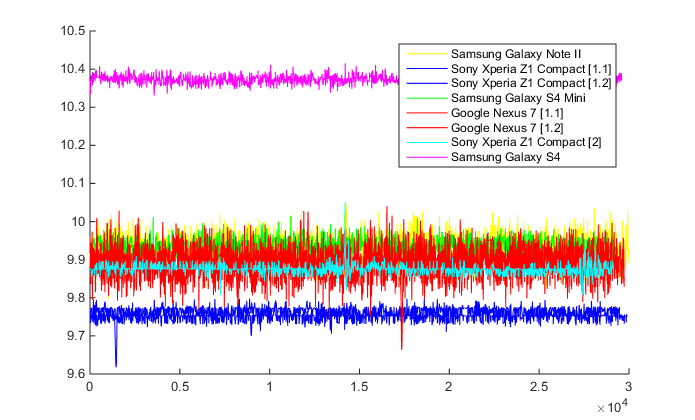
\includegraphics[scale=.7]{img/oneMonth-plot-RMS}
	\caption{Scatter graph on accelerometer recordings of 6 Android devices, where two has one month apart}
	\label{fig:plot1mRMS}
\end{figure}

% ========== CAMERA TEST ==========
\section{Result Camera-test}\label{sec:ResCam}
\textbf{ ==== OBS!! ====}\\ Flyttad text som måste skrivas om.
For the test of the camera sensor the PRNU value is calculated as an approximation of the algorithm described in section ~\ref{sec:char:camera} and also used by \cite{sensor:camera:DCIdent}. That is the average of multiple pictures used and substantially an approximation of \textit{f}. The first step is to remove the pictures-content which leaves the noise, which is done using a denoising filter. For the test the MATLAB \texttt{medfilt2} is used, which is an 2-D median filtering that outputs the median value of each pixel by its 3-by-3 neighbors. 
\begin{figure}[H]
  \centering
  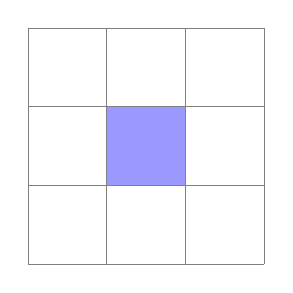
\begin{tikzpicture}[scale=1]
	\draw[step=1cm,gray,very thin] (0,0) grid (3,3);
	\fill[blue!40!white] (1,1) rectangle (2,2);
\end{tikzpicture}
  \caption{\label{fig:medfilt2} the MATLAB \texttt{medfilt2} outputs the median of each pixel by it's 3-by-3 neighbors}
\end{figure}
From the \texttt{medfilt2} we gain a picture without noise which is then subtracted from the original to get the noise. This technique works best if there are no features on the pictures such auto-fix, black and white etc. The more images used for the average value the better noise is, thus the amount random noise is less and the fixed noise is more. \cite{sensor:camera:DCIdent} recommend a minimum of 50 images. This is then seen as the reference pattern used for correlating the noise from another pictures. This correlation is calculated like:
$$
corr(\boldsymbol{n},\boldsymbol{r}) = 
\frac{(\boldsymbol{n} - \bar{\boldsymbol{n}})(\boldsymbol{r} - \bar{\boldsymbol{r}})}
{\|\boldsymbol{n} - \bar{\boldsymbol{n}}\| \|\boldsymbol{r} - \bar{\boldsymbol{r}}\|}
$$
A threshold for acceptance on correlation is found by experimental on images taken with or without the camera. Then there is a balance between FAR and FRR. 
In section ~\ref{sec:measurement:camera} i described two test preformed on the camera sensor of mobile devices.
\subsection{Test I}
Since the purpose of this thesis compared to earlier work REFERENSER!! has the purpose of authentication and not forensics, is convenience for the collecting and measurability a factor to take in account. That is why the fist experiment is asked the users to record a 5 seconds video-clip with the device camera facing down on a flat object, like a table. Instead of making the user take 50 pictures or more which takes a lot of more time. This also makes it easier to get better noise since the same scene is used every time. \\
The video is then shuttled into images (100-200 from a 5 seconds video depending on fps on recording camera) that is used for calculating the PRNU. The MATLAB code for this is:\\
\rule{\textwidth}{0.5pt}
  \lstinputlisting{code/video2prnu1.m}
\rule{\textwidth}{0.5pt}

To compare an pictures between all collected PRNU the same calculation to get the noise is done. Then the noise from the reference pictures is compared to all collected PRNU and correlation is calculated like the formula above in MATLAB:\\
\rule{\textwidth}{0.5pt}
  \lstinputlisting{code/corrCamTest1.m}
\rule{\textwidth}{0.5pt}

\subsection{Test II}
Since the earlier test leaved out some of the PRNU noise when recorded a video instead of taking a picture the new test consist of 10 images from every device. The recommendation from \cite{sensor:camera:DCIdent} to use at least 50 images is here compensated by again using black images (picture taking with device camera facing down). Since the scene is always the same the noise removal will be better in fewer images. The same code is used as above with the different that the video to image step is removed. The sizes of the images in this case is better since the camera on the mobile devices by default uses higher resolution when taking a picture then when recording. 

